\documentclass[11pt]{article}
\usepackage{amsmath, amsfonts}
\usepackage{graphicx}
\graphicspath{images/}


\begin{document}


%\chapter{Asset Liability Management (ALM)}
%\section{}
%
%This chapter introduces the usage of R for commercial bank \textbf{asset and liability management (ALM)} purposes. The ALM function in a bank is traditionally associated with interest rate risk and liquidity risk management of banking book positions. Both of the interest rate positioning and liquidity risk management require the modeling of banking products. Nowadays, professional ALM units use complex \textbf{Enterprise Risk Management (ERM)} frameworks, which are able to incorporate the management of all risk types and provide an adequate tool for ALM to steer the balance sheet. Our general objective is to set up a simplified framework of ALM to illustrate the use of R for certain ALM tasks. These tasks are based on the interest rate and liquidity risk management and the modeling of non-maturing accounts.
%
%
%This chapter is structured as follows. We start with the data-preparation process of
%ALM analysis. The process of planning and measurement needs special information
%about the banking book, market conditions, and the business strategy. This part
%establishes a data-management tool that consists of the major input datasets, and
%extracts data into the form that we use in the rest of this chapter.
%
%
%Next, we will be dealing with the measurement of the interest rate risk. There are
%two common approaches in the banking industry to quantify interest rate risk in
%the banking book. Simpler techniques use repricing gap table analysis to manage
%the interest rate risk exposure and calculate parallel yield curve shocks to forecast
%the net \textbf{interest income (NII) }and calculate the \textbf{market value of equity (MVoE)}.
%More advanced methods use dynamic simulation of balance sheets and stochastic
%simulation of interest rate development. Choosing which tool to use depends on the
%targets and the balance sheet structure. 
%
%
%For example, a savings bank (with client term deposits on the liability side and fix
%bond investments on the asset side) focuses on its market value of equity risk, while
%a corporate bank (with floating interest position) concentrates on the net interest
%income risk. We illustrate how to efficiently provide a repricing gap table and net
%interest income forecasts with Python.
%
%In the last section of this chapter, we will concentrate on the modeling of non-maturing
%products. Client products can be classified by their maturity structure and interest
%rate behavior. Examples of typical non-maturing liability products are on-demand
%deposits and savings accounts without any notice period of withdrawal. The clients
%can withdraw their money at any time, while the bank has the right to modify the
%offered interest rate. On the asset side, overdrafts and credit cards show quite similar
%characteristics. The complex models of non-maturing products make the work of ALM
%quite challenging. Practically, the modeling of non-maturing products means
%the mapping of the cash-flow profiles, estimating the interest rate elasticity of the
%demand, and analyzing the liquidity-related costs in the internal funds transfer
%pricing (FTP) system. Here, we demonstrate how to measure the interest sensitivity
%of the non-maturing deposits.


%%%%%%%%%%%%%%%%%%%%%%%%%%%%%%%%%%%%%%%%%%%%%%%%%%%%%%%%%%%%%%%%%%%%%%%%%%%%%%%%%%
%%%%%%%%%%%%%%%%%%%%%%%%%%%%%%%%%%%%%%%%%%%%%%%%%%%%%%%%%%%%%%%%%%%%%%%%%%%%%%%%%%


%TODO Introduction'
%TODO Data description'
%TODO Loans'
%TODO Yield curve'
%TODO Cashflows'
%TODO Interest rate risk measurement'




\section{Introduction}


\subsection{Background}

Asset and Liability Management (ALM) is a mechanism to address the risks faced by a
bank that arise as a result of a mismatch between assets and liabilities due to liquidity and changes in interest rates. One of the central issues of ALM is to manage interest rate risk associated with long-term and non tradable assets and liabilities. ALM focuses on bank’s earnings and value which aim to measure the interest rate risk in the banking book.


The phrase ’interest rate risk in the banking book’ (IRRBB) implies that the bank’s position and its financial situation are sensitive to fluctuations in market interest rates.\\


Currently, regulators are considering standardizing the management of IRRBB to a certain extent. An example of a step taken in this direction are the reporting standards
to IRRBB proposed by Basel Committee on Banking Supervision (BCBS) which were
issued in April 2016 with the title: ”Standards on Interest Rate Risk in the Banking
Book”. The new reporting standards propose two perspectives on evaluating IRRBB:
earnings and economic value. The earnings perspective focuses on the impact of interest rate movements on the net interest or accrued income of a bank over a time
horizon of several years. This perspective is measured in terms of Net Interest Income
(NII). The economic value perspective focuses on the impact of changes in interest rate
movements on the value of an institution’s asset, liabilities and off-balance sheet items.\\


This perspective is measured in terms of Economic Value of Equity (EVE) (BCBS,
2016). These two perspectives are based on different concepts, yield different results
and employ different interest rate risk strategies.
The earnings perspective captures the short-term effect of interest rate changes, whereas
the economic value perspective captures the long-term effect of interest rate changes.
Therefore, the two perspectives are considered complementary. As such, regulators
require banks to disclose both metrics, in order to enable comparability. These two
perspectives however follow different procedures and lead to different outcomes. Nevertheless, these two perspectives cannot be considered separately either. A pure focus on one could lead to destabilization of the alternative resulting in a trade-off.



%%%%%%%%%%%%%%%%%%%%%%%%%%%%%%%%%%%%%%%%%%%%%%%%%%%%%%%%%%%%%%%%%%%%%%%%%%%%%%%%%%
%%%%%%%%%%%%%%%%%%%%%%%%%%%%%%%%%%%%%%%%%%%%%%%%%%%%%%%%%%%%%%%%%%%%%%%%%%%%%%%%%%

\section{Data Description}

For the interest rate risk modelling part, we use two datasets from $2014-09-30$, namely the bank's portfolio and the market for zero-coupon bonds with different maturities.\\

More specifically, the portfolio contains the following data. 
\begin{itemize}
	\item \textit{id:} identification number (index of the row)
	\item \textit{account:} account type in short (e.g. mmp\_1)
	\item \textit{account\_name:} long account name (e.g. Money market placements)
	\item \textit{volume:} notional value in EUR
	\item \textit{ir\_binding:} type of the interest rate. FIX for fixed rates, and LIBOR for variable rates with the variable benchmark LIBOR
	\item \textit{reprice\_freq:} repricing frequency (of the rates) in months if the interest binding is LIBOR
	\item \textit{spread:} the spread component of the interest rate in basis points (1 basis point $0.01\%$). The other component is the market's interest rates. $$(\text{Interest rate}) = (\text{Market's interest rate})+(\text{spread})$$
	\item 
\end{itemize}

    
%    - Cash-flow structure of the products
%    :col issue: issue date (this is the first repricing day)
%    :col maturity: maturity date
%    :col repayment: type of principal repayment structure (bullet, linear, or annuity)
%    :col payment_freq: repayment frequency in number of months
%    :col yieldcurve: identifier of the interest rate curve

%%%%%%%%%%%%%%%%%%%%%%%%%%%%%%%%%%%%%%%%%%%%%%%%%%%%%%%%%%%%%%%%%%%%%%%%%%%%%%%%%%
%%%%%%%%%%%%%%%%%%%%%%%%%%%%%%%%%%%%%%%%%%%%%%%%%%%%%%%%%%%%%%%%%%%%%%%%%%%%%%%%%%

\section{Amortization Schedule}

When a bank gives out a loan, the loan is expected to be payed back with interest. An \textbf{amortizing loan} is a type of loan in which the borrower makes regular, periodic payments that include both \textbf{principal} and \textbf{interest}. These payments are structured in a way that ensures the full repayment of the original loan amount (the principal) along with all accrued interest by the end of the loan term, or \textbf{maturity}. The process of spreading out the repayment of a loan over time is called \textbf{amortization}. The term "amortize" means to gradually reduce or pay off a debt over time.\\

The \textbf{amortization schedule} is a table or spreadsheet that outlines the details of each payment, including the amount allocated to principal and interest for each period. It also shows the remaining balance after each payment. This schedule provides borrowers with a clear understanding of how their loan will be paid off and helps them budget for future payments. On the other side, for the banks the amortization schedule is useful for the calculations of future cashflows for risk management.

\subsection{Loan Payment Structure}

In this section we describe three basic and frequent loan payment structures, namely, the linear, the annuity and finally the bullet. The names describe the distribution of principal payments (repayment of the original loan volume). For example, for the linear loan payment, every month we pay fixed amount on the principal value. 


\subsubsection{Bullet Loan Payment Structure}

A bullet loan, also known as a bullet payment loan or balloon payment loan, is a type of loan structure in which the borrower makes regular interest payments throughout the loan term but repays the entire principal (the original loan amount) in a single lump-sum payment at the end of the loan term.\\

Suppose $P$ represents the principal amount, and the loan is to be repayed in $N$ regular (e.g. monthly) instalments. If at each period $i$, the interest rate (for the length of this period) is $r_i$, then the payment for that period $p_i$ is 
\begin{align}
	p_i(P,r_i,N) =r_i\cdot P+\delta_{i,N}\cdot P
	\label{bullet}
\end{align}
with $r_i\cdot P$ being the interest payment, and $\delta_{i,N}\cdot P$ is the final lump-sum principal payment.
\begin{figure}[ht!]
	\centering
	\begin{tabular}{|c|c|c|c|c|}
		\hline
		& cashflow & interest & capital & remaining\\
		\hline
		1 & 75.0 & 75.0 & 0.0 & 7500.0\\
		\hline
		2 & 75.0 & 75.0 & 0.0 & 7500.0\\
		\hline
		3 & 7575.0 & 75.0 & 7500.0 & 0.0\\
		\hline
	\end{tabular}
	\caption{Example of amortization schedule for a bullet loan with principal volume $7500$, monthly rate $0.01$ and maturity 3 months after issuance.}
\end{figure}

	


\subsubsection{Linear Payment Structure}

A linear loan, also known as a straight-line loan or linear amortizing loan, is a type of loan structure in which the borrower pays back an equal portion of the principal at each payment period, along with the interest on the outstanding balance. The principal repayment remains constant throughout the loan term. However, since the outstanding balance reduces with each payment, the interest portion decreases over time, making the total payment amount decline over the life of the loan.\\

Suppose $P$ represents the principal amount, and the loan is to be repayed in $N$ regular (e.g. monthly) instalments. If at each period $i$, the interest rate (for the length of this period) is $r_i$, then the payment for that period $p_i$ is 
\begin{align}
	p_i\big(P,N,r_i,\{p_j\}_{j=1}^{i-1}\big)= \frac{P}{N}+r_i\cdot\underbrace{\bigg[P-\sum_{j=1}^{i-1}p_j\bigg]}_{\text{outstanding bal.}}
	\label{linear}
\end{align}
The first term is the principal payment, while the second is the interest payment.
\begin{figure}[ht!]
	\centering
	\begin{tabular}{|c|c|c|c|c|}
		\hline
		& cashflow & interest & capital & remaining\\
		\hline
		1 & 2575.0 & 75.0 & 2500.0 & 7500.0\\
		\hline
		2 & 2550.0 & 50.0 & 2500.0 & 5000.0\\
		\hline
		3 & 2525.0 & 25.0 & 2500.0 & 2500.0\\
		\hline
	\end{tabular}
	\caption{Example of amortization schedule for a linear loan with principal volume $7500$, monthly rate $0.01$ and maturity 3 months after issuance.}
\end{figure}



\subsubsection{Annuity Payment Structure}

An annuity payment structure refers to a series of periodic payments made at equal intervals. The key feature of this payment structure is that the sum of the present values of all payments must be equal to the principal value. When the interest rates are fixed, the borrower makes equal total payments each period consisting of both principal and interest. At the beginning of the loan term, a large portion of each payment is applied to interest, with a smaller portion going to reduce the principal. As the loan matures, the interest portion of each payment decreases, and the principal portion increases, but the total payment remains the same.\\

Suppose $P$ represents the principal amount, and the loan is to be repayed in $N$ regular (e.g. monthly) instalments. If at each period $i$, the interest rate (for the length of this period) is $r_i$, then the payment for that period $p_i$ is derived in the following fashion.\\

An annuity is a series of constant (fixed) payments (or cash flows) of $p_i=p$ made at the end of each period over $n$ periods. To derive the formula for $p_i$, we consider the present value of each payment. If we make the payment on the $i$th payment period, its present value is 
$$\text{PV}(p_i)=p\bigg/\prod_{j=1}^i(1+r_j)$$
The present value of all the payments is required to be equal to the principal value of the loan. That is,
\begin{align}
	P=\sum_{i=1}^N\text{PV}(p_i)=p\sum_{i=1}^N\bigg[\prod_{j=1}^i(1+r_j)\bigg]^{-1}\nonumber
\end{align}
which gives us 
\begin{align}
	p_i=P\bigg/\sum_{i=1}^N\bigg[\prod_{j=1}^i(1+r_j)\bigg]^{-1}\label{annuity_der}
\end{align}
When the interest rates are fixed, the formulas become much simpler. To be more explicit

$$P=p\cdot \sum_{i=1}^N\frac{1}{(1+r)^i}=p\cdot\frac{1-(r+1)^{-N}}{r}$$
and therefore, we find that the constant periodic payment is
\begin{align}
	p(P, N, r)=\frac{r\cdot P}{1-(1+r)^{-N}}\label{annuity_payment}
\end{align}
\\

In all practical cases, when the interest rates are variable, the payment is not calculated with \eqref{annuity_der}, because, even thought the future interest rates may be predicted under certain models and assumptions, they are not known. In this case, the periodic payment is not constant and is recalculated at each period based on the current interest rate, the outstanding balance, and the time to maturity at that time with \eqref{annuity_payment}. Thus, the payment (or cashflow) during the $i$th payment period is
\begin{align}
	p_i=\frac{r_i}{1-(1+r_i)^{-N_i}}\cdot \underbrace{\bigg [P-\sum_{j=1}^ip_j\bigg]}_{\text{outstanding bal.}}
	\label{annuity}
\end{align}
with $N_i$ being the number of payment periods remaining to maturity. The payment on each due date is determined as though the loan began on that specific date, using the remaining balance as the principal amount and applying the current floating rate, which is presumed to continue until the loan's end date.
\begin{figure}[ht!]
	\centering
	\begin{tabular}{|c|c|c|c|c|}
		\hline
		& cashflow & interest & capital & remaining\\
		\hline
		1 & 1922.11 & 75.0 & 1847.11 & 5652.89\\
		\hline
		2 & 1922.11 & 56.53 & 1865.58 & 3787.30\\
		\hline
		3 & 1922.11 & 37.87 & 1884.24 & 1903.10\\
		\hline
	\end{tabular}
	\caption{Example of amortization schedule for a linear loan with principal volume $7500$, monthly rate $0.01$ and maturity 3 months after issuance.}
\end{figure}

\textit{The cashflow.py module includes a function named amortization\_schedule. This function provides the amortization schedule for an asset or liability, offering repayment structures such as bullet, linear, or annuity, as demonstrated in prior examples.}
%%%%%%%%%%%%%%%%%%%%%%%%%%%%%%%%%%%%%%%%%%%%%%%%%%%%%%%%%%%%%%%%%%%%%%%%%%%%%%%%%%%%%%%%%%%%%%%
%%%%%%%%%%%%%%%%%%%%%%%%%%%%%%%%%%%%%%%%%%%%%%%%%%%%%%%%%%%%%%%%%%%%%%%%%%%%%%%%%%%%%%%%%%%%%%%

\section{Yield Curve}

A \textbf{yield curve} is a graphical representation of annual returns on assets with similar risk profile for a range of maturities. The horizontal axis represents the time to maturities, while the vertical axis represents the yield.

\subsection{Spot yields}

 In our case, we are interested in \textbf{spot yields} or \textbf{spot rates}, which are the yields of zero-coupon bonds for specific maturities. A \textbf{zero-coupon bond} is a bond that does not make periodic interest payments and is instead issued at a discount too its face value. It matures at its face value, and the difference between the purchase price and that face value is the interest earned by the bondholder.\\
 
 Since spot yields pertain to zero-coupon bonds, they provide a pure measure of interest rates over different horizons without the complexities introduced by periodic coupon payments. This makes them a clear and direct indicator of the cost of borrowing money for specific time periods. \\
 
  Spot yields are useful to banks for a number of reasons; for example loan pricing and deriving forward rates. As far as the loan pricing is concerned, banks might refer to the yield curve and issue loans with rate calculated by adding a spread to the spot yield for the corresponding maturity, for credit-risk and profit. As for the forward yields, we describe them in a following subsection.


\subsection{Modelling Spot Yield Curve}

One can find the relation between the spot yields and the time to maturity with various models. A particularly flexible model is the  Nelson--Siegei--Svensson model. \\

The Nelson and Siegel group of models are based on the original model by Nelson and Siegel, which originally had four parameters. The Svensson extension introduced two new “slope” parameters to allow for a better variety of shapes for both instantaneous forward rate curves and yield curves.  Virtualy any yield curve shape can be interpolated using these two models, which are widely used at banks around the world.\\

Two of the main reasons we want to model the relation between the time to maturity and the spot yield are interpolation, and extrapolation.
Sometimes there are missing values in a time-series data set. For instance, interest rates for years 1 to 3 may exist, followed by years 5 to 8, and then year 10. Our model can be used to also be used to forecast or extrapolate values of future time periods beyond the time period of available data.\\

The known $x$ values represent the values on the $x$-axis, which are the values that are known in advance such as time (or years). and the known $y$ values represent the values on the $y$-axis (in our case, the known Interest Rates). The $y$-axis variable is typically the variable you wish to interpolate missing values from or extrapolate the values into the future.\\

 Equation \eqref{nss_instantaneous_forward_rate} shows how the instantaneous forward rate can be expressed as a function of the six parameters. The Nelson-Siegel-Svensson model provides a well behaved, smooth forward rate curve. The original Nelson-Siegel model is the same as the Svensson with $\beta_4=0$. Equation \eqref{nss_closed_form} shows how the model can be expressed as a closed form expression of yields.
\begin{align}
	f(t)=\beta_1+\beta_2\exp\bigg(\frac{-t}{\lambda_1}\bigg)
			+\beta_3\frac{t}{\lambda_1}\exp\bigg(\frac{-t}{\lambda_1}\bigg)
			+\beta_4\frac{t}{\lambda_2}\exp\bigg(\frac{-t}{\lambda_2}\bigg)
			\label{nss_instantaneous_forward_rate}
\end{align}
\begin{align}
	r(t)=\beta_1&+\beta_2\bigg(\frac{t}{\lambda_1}\bigg)^{-1}\bigg[1-\exp\bigg(\frac{-t}{\lambda_1}\bigg)\bigg]\nonumber\\
		&+\beta_3\bigg\{\bigg(\frac{t}{\lambda_1}\bigg)^{-1}\bigg[1-\exp\bigg(\frac{-t}{\lambda_1}\bigg)\bigg]-\exp\bigg(\frac{-t}{\lambda_1}\bigg)\bigg\}\nonumber\\
		&+\beta_4\bigg\{\bigg(\frac{t}{\lambda_2}\bigg)^{-1}\bigg[1-\exp\bigg(\frac{-t}{\lambda_2}\bigg)\bigg]-\exp\bigg(\frac{-t}{\lambda_2}\bigg)\bigg\}
		\label{nss_closed_form}
\end{align}
A benefit of the Nelson-Siegel-Svensson model is the interpretations of $\beta_1$ and $\beta_1+\beta_2$. $\beta_1$ can be interpreted as the long term interest rate, while $\beta_1+\beta_2$ is the instantaneous short term interest rate.

 \subsection{Forward Yields}

Forward yields (or forward rates) represent the expected future interest rates for specific periods, derived from current spot rates. They offer insight into the market's expectations regarding future interest rate movements, economic conditions, and expected future cashflows. Forward rates can be calculated under the assumption of non-arbitrage with the following syllogism. 

Suppose we aim to determine the forward yield \(f_{t,s}\) for a zero-coupon bond that begins accruing in \(t\) periods (e.g., years) and spans \(s\) periods. To find \(f_{t,s}\), we set up a scenario. Imagine we first invest in a bond maturing in \(t\) periods with a current spot yield of \(Y_t\). Once this bond matures, we then reinvest the proceeds into a new zero-coupon bond that starts accruing at \(t\) and matures at \(t+s\). The return from this strategy should be equivalent to directly investing in a zero-coupon bond that begins accruing now and matures at \(t+s\) with a spot yield of \(Y_{t+s}\). Therefore, the relationship can be expressed as:
\begin{equation}
(1 + Y_{t+s})^{t+s} = (1 + Y_t)^t(1 + f_{t,s})^s
\end{equation}
From which, the forward yield \(f_{t,s}\) can be isolated as:
\begin{equation}
f_{t,s} = \left[ \frac{(1 + Y_{t+s})^{t+s}}{(1 + Y_t)^t} \right]^{1/s} - 1
\label{forward_rates}
\end{equation}


\textit{The yieldcurve.py module includes a YieldCurve class that is fits the Nelson-Siegei-Svensson model to market data, and subsequently can provide spot rates and forward rates for provided dates and time periods. Additionally, given repricing dates, it can return the floating rates for certain payment dates.
}

\section{Portfolio Cashflows}

In this section, we detail the methodology for calculating the bank's portfolio cashflows. We previously emphasized that the portfolio encompasses both assets and liabilities. Moreover, we clarified that all assets have one of three repayment structures: bullet, linear, or annuity. The cashflows for these assets and liabilities are determined using equations \eqref{bullet}, \eqref{linear}, and \eqref{annuity}, provided we apply the appropriate rates. Some items bear fixed interest rates, making their generated cash flows resistant to interest rate changes. Conversely, variable-rate items adjust according to interest rates. To forecast their future cash flows, it's essential to know the rate values on upcoming payment dates. Although exact predictions are challenging, we can make estimations using forward rates from the yield curve, as indicated in equations \eqref{nss_closed_form} and \eqref{forward_rates}.

\subsection{Floating Rates}


Suppose we aim to forecast future cashflows for an asset influenced by variable rates, using LIBOR as a benchmark, and an added spread \(s\) on top. This asset has an issuance date of \(d_i\) and matures on \(d_m\). Our dataset includes the repayment frequency, denoted in months as \(T_{\text{repay}}\). We use this frequency to determine repayment dates by moving backwards from the maturity date in intervals set by the repayment frequency:
$$D_{pay}=\{d_{pay}=d_m-j\cdot T_{repay}\ |\ j\in \mathbb{N}\ \wedge\ d_{pay}\geq d_i\}$$
Furthermore, our data indicates the repricing frequency in months as \(T_{\text{reprice}}\). This frequency helps establish the dates when the asset's interest rates are revised. The initial rate is set on the issuance date \(d_i\), with subsequent adjustments happening every \(T_{\text{reprice}}\) months:
 $$D_{reprice}= \{d_{reprice}=d_i+j\cdot T_{reprice}\ |\ j\in\mathbb{N}\ \wedge\ d_{reprice} \leq d_m\}$$

The interest rate remains unchanged between successive repricing dates. To estimate these forthcoming rates, forward rates tailored for each duration are utilized. Consider $P_j$ as the interval from the $j$th to the $(j+1)$th repricing date, defined as
$$P_j=[d_{reprice}(j),\ d_{reprice}(j)+T_{reprice})$$
Let's introduce a function \(y(d_1,d_2)\) that calculates the difference in years between two dates, starting from \(d_1\) and concluding on \(d_2\). Using \(d_{\text{today}}\) to represent the present date, we can express \(t_j\) as \(y(d_{\text{today}},d_{\text{reprice}}(j))\). For the interval \(P_j\), the benchmark LIBOR rate is presumed to be invariant, aligning with the forward rate:
\begin{align}
	f_{t_j,s}=\left[ \frac{(1 + Y_{t_j+s})^{t_j+s}}{(1 + Y_{t_j})^{t_j}} \right]^{1/s} - 1	
\end{align}
where \(s\) stands for \(T_{\text{reprice}}\) expressed in years. To find the annual interest rate of the asset or liability, we simply add the corresponding spread to $f_{t_j,s}$.\\

Finally, for each payment date \(d_{\text{pay}}\in D_{\text{reprice}}\), we determine the period \(P_j\) such that \(d_{\text{pay}}\in P_j\), and assign the corresponding rate to it. With these rates then, we can calculate the cashflow from each asset or liability with \eqref{bullet}, \eqref{linear} or \eqref{annuity}, depending on its repayment structure.\\

\textit{In the cashflow.py module, the asset\_cashflow function provides cashflows for an individual asset or liability, distinguishing between interest and principal components. Additionally, the portfolio\_cashflow function delivers cashflows for every asset or liability within the portfolio.}



\section{Interest Rate Risk}

Interest rate risk is the potential for changes in interest rates to negatively impact the financial position of an institution, particularly those institutions that are involved in lending, borrowing, or holding fixed-income securities. Interest rate management focuses on the sensitivity of \textbf{net interest income (NII)}.  The net interest income equals the difference between interest revenues and interest expenses.\\

Assume $\mathcal{A}_S$ and $\mathcal{A}_{NS}$ be the sets of interest sensitive and non-sensitive assets. Similarly, let $\mathcal{L}_S$ and $\mathcal{L}_{NS}$ be the sets of interest sensitive and non-sensitive liabilities. Then the net interest income is
\begin{align}
	\text{NII}=\sum_{a_S\in\mathcal{A}_S}R(a_S)+\sum_{a_{NS}\in\mathcal{A}_{NS}}R(a_{NS})-\sum_{l_S\in\mathcal{L}_{NS}}R(l_S)-\sum_{l_{NS}\in\mathcal{L}_{NS}}R(l_{NS})
\end{align}
with $R$ symbolising the interest component of cashflows from the asset $a$ or liability $l$.\\


\textit{The \textit{cashflow.py} module contains a function \textit{nii\_table} that returns a table with the annual NII for each account name in the portfolio, as well as the totals. It additionally plots a bar plot for the data.} \\


 The traditional approach of interest rate risk positioning of the balance sheet is based on \textbf{gap} models. \textbf{Interest rate gap} refers to the net asset position for a certain time period between interest-bearing assets and liabilities, which are repriced at the same time. The interest rate gap ($G$) equals:
\begin{align}
	G=\sum_{a_S\in\mathcal{A}_S}V(a_S)-\sum_{l_S\in\mathcal{L}_S}V(l_S)
\end{align}
where $V$ gives the volume of the interest sensitive assets or liabilities.We can categorize the assets and liabilities in the book that bear interest risk based on their month of repricing. This table is termed the \textbf{repricing gap table}. A bar plot representing this for the upcoming 12 months can be seen in Figure \ref{repricing_gap_table}.\begin{figure}[ht!]\label{repricing_gap_table}
	\centering
	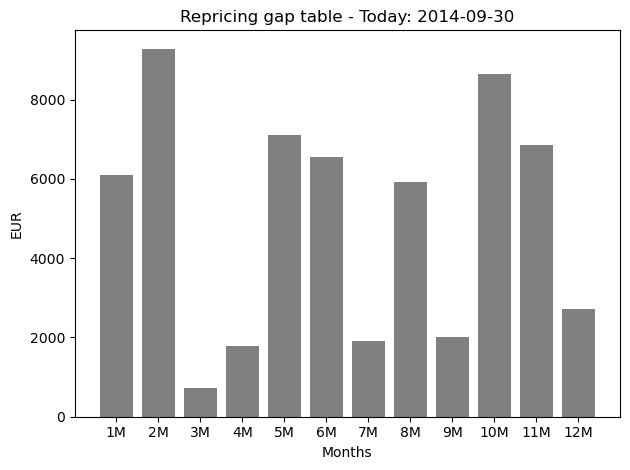
\includegraphics[scale=0.4]{images/reprGapTable}	
	\caption{Repricing gap table for the 12 upcoming months.}
\end{figure}\\

\textit{The cashflow.py module contains a function repricing\_gap\_table, which creates the repricing gap table, and optionally plots the values for a number of upcoming months.}
\\

\textbf{Interest earnings variation} can be characterized as the risk-bearing items multiplied by the change of interest rate $\Delta i$, shown as follows:
\begin{align}
	\Delta\text{NII}=G\cdot \Delta i
\end{align}

The sign of the gap is crucial from an interest rate risk point of view. A positive
gap indicates increasing earnings when interest rates rise, and indicates decreasing earnings when interest rates decline. The repricing gap table can also capture the basis risk by aggregating the interest-bearing assets and liabilities based on their reference interest rate (that is 3 months or 6 months EURIBOR). Interest rate gap tables can be sufficient tools to determine the risk exposure from the earnings perspective. However, gap models cannot be used as a single risk measure to quantify rather the net interest income risk of the total balance sheet. Interest rate gaps are management tools, which provide guidance on interest rate risk positioning.\\

We have to mention that there are more sophisticated tools for interest rate risk management. In practice, simulation models are applied for risk management purposes. However, the banking book risks are not explicitly subjected to capital charge under Pillar 1 of the Basel II regulations; Pillar 2 covers the interest rate
risk in the banking book. Regulators lay particular emphasis also on the risk assessment regarding the market value of equity. Risk limits are based on specific stress scenarios, which could be either deterministic interest rate shocks or historical volatility-based earnings at risk concepts. Therefore, risk measurement techniques stand for scenario-based or stochastic simulation approaches, focusing on the interest earnings or the market value of equity. Net interest income simulation is rather a dynamic, forward-looking approach, while calculation of the market value of equity provides a static result. Equity duration is also a widely used measure for interest rate risk of the banking book. Duration of the assets and liabilities are calculated
to quantify the duration of equity. ALM professionals often use effective duration, which incorporates embedded options (caps, floors, and so on) in the interest rate sensitivity calculation.



\section{Liquidity Risk}

Traditionally, liquidity risk is measured with two primary tools - static and dynamic liquidity gap tables. These tools help banks understand their liquidity position, i.e., their ability to meet short-term obligations with available cash or near-cash assets.\\

 \textbf{Liquidity gap tables} essentially a representation of the bank's balance sheet, but instead of organizing assets and liabilities by type (e.g., loans, deposits), they are organized by when they are expected to result in cash \textbf{inflows} (expected incoming cash flows, like loan repayments from customers or interest payments) or \textbf{outflows} (expected outgoing cash flows, like withdrawals by depositors or maturing debt the bank needs to repay). This is done using "\textbf{maturity buckets}," which could be time periods like "less than 1 month," "1-3 months," "3-6 months," and so on. For each maturity bucket, the n\textbf{et cash-flow gap} is calculated by subtracting expected outflows from expected inflows. A positive gap indicates that the bank expects more inflows than outflows for that period, while a negative gap suggests potential liquidity shortfalls.\\
 
As mentioned above, there are two approaches; the static and the dynamic. The \textbf{static} approach assumes a "rundown" balance sheet, meaning it only considers existing contracts and obligations without factoring in potential new business or the possibility of existing contracts being renewed. It's a snapshot based on current conditions.
The \textbf{dynamic} is a more comprehensive approach. It considers not just the current balance sheet but also potential future scenarios. For instance, a loan might be rolled over (renewed), or the bank might acquire new deposits or make new loans. This view tries to account for these possibilities, making it more complex but also more realistic.
For simplicity, in what follows, we adopt the static view.




\section{Non-maturity deposits}

The importance of \textbf{non-maturity deposits (NMD)} in banking is substantially high as the large part of commercial banks' balance sheets consist of client products with non-contractual cash-flow features. Non-maturity deposits are special financial instruments as the bank has an option to change the paid interest on the deposit account at any time, and the client has the option to withdraw any amount from the account without a period of notice. The liquidity and interest rate risk management of these products are a crucial part of ALM analysis; therefore, modeling of non-maturity deposits needs special attention. The uncertain maturity and interest rate profile generates a high level of complexity in their hedging, internal transfer pricing, and risk modeling.
\\

In the following analysis, we use Austrian non-maturity deposit time series data that we queried from the ECB Statistical Database, which is publicly available. We have monthly deposit interest rates (cpn), end-of-month balances (bal), and the 1 month EURIBOR fixing (eur1m) in our dataset.
\begin{figure}[ht!]
	\centering
	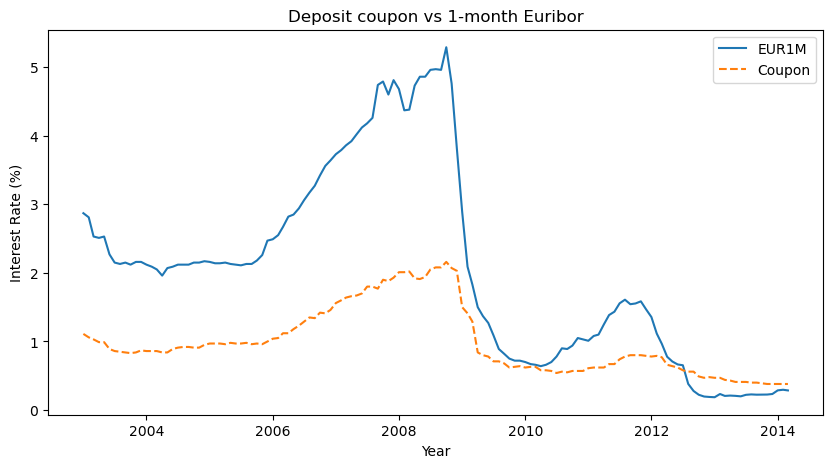
\includegraphics[scale=0.6]{images/cpn_erb}
	\caption{Deposit coupon and 1 month EURIBOR fixing with time.}	
\end{figure}

\subsection{Relationship between 1-month EURIBOR and Deposit Interest Rates}

We aim to investigate the relationship between two time series: the 1-month EURIBOR fixing and deposit interest rates. Specifically, we want to understand the long-term influence of the 1-month EURIBOR rate on non-maturity deposit interest rates. The concept of the 'pass-through effect' describes how fluctuations in the EURIBOR influence deposit interest rates. If there's a full pass-through, then a change of $\delta$ in the EURIBOR would lead to an equivalent $\delta$ change in deposit rates. Given its significance in assessing market dynamics, regulators, including the ECB, have emphasized understanding this effect. The ECB has even mandated that banks in the euro-zone gauge this pass-through effect under certain stress-testing conditions.




We use the Engle-Granger two-step method to estimate the ECM model. In the first step, we estimate the cointegrating vector with a regression model. We take the residuals, and in the second step, we estimate the long-term and short-term effects of EURIBOR on deposit rates using the error-correction mechanism. Before the first step, we have to test whether both time series are integrated in the same order. Therefore, we run Augmented Dickey-Fuller (ADF) and the KPSS tests

\subsubsection{}



\end{document}
